\documentclass[tikz,border=10pt]{standalone}
\usetikzlibrary{arrows.meta}
\pagecolor{white}
\begin{document}
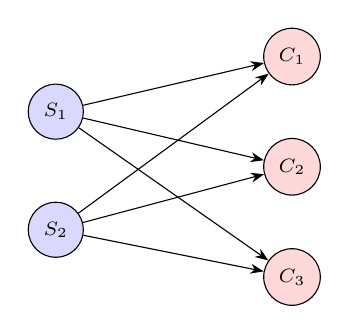
\begin{tikzpicture}[
  sup/.style={circle,draw,fill=blue!15,minimum size=0.7cm,font=\scriptsize\bfseries},
  cus/.style={circle,draw,fill=red!15,minimum size=0.7cm,font=\scriptsize\bfseries},
]
  \node[sup] (s1) at (0, 1.5) {$S_1$};
  \node[sup] (s2) at (0, 0)   {$S_2$};
  \node[cus] (c1) at (3, 2.2) {$C_1$};
  \node[cus] (c2) at (3, 0.8) {$C_2$};
  \node[cus] (c3) at (3,-0.6) {$C_3$};
  \foreach \s in {s1,s2}
    \foreach \c in {c1,c2,c3}
      \draw[-{Stealth},thin] (\s) -- (\c);
\end{tikzpicture}
\end{document}
